\documentclass[tikz, border=3mm]{standalone}
\usepackage{tikz}
\usetikzlibrary{arrows.meta}

\begin{document}
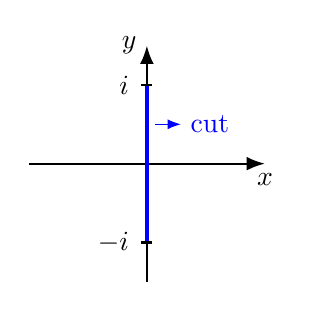
\begin{tikzpicture}[
    >=Latex, % Set default arrow tip style
    tick/.style={thick} % Style for tick marks
]

% Axes
\draw[->, thick] (-1.5, 0) -- (1.5, 0) node[below] {$x$};
\draw[->, thick] (0, -1.5) -- (0, 1.5) node[left] {$y$};

% Vertical Cut Line
\draw[blue, ultra thick] (0, -1) -- (0, 1);

% Ticks on the y-axis for the cut endpoints
\draw[tick] (-2pt, 1) -- (2pt, 1); % Tick at y=1
\draw[tick] (-2pt, -1) -- (2pt, -1); % Tick at y=-1

% Endpoint Labels (adjusted slightly for ticks)
\node[left=3pt] at (0, 1) {$i$};
\node[left=3pt] at (0, -1) {$-i$};

% Cut Label and Arrow
\node[blue] (cutlabel) at (0.8, 0.5) {cut}; % Position the text label
\draw[->, blue] (0.1, 0.5) -- (cutlabel.west); % Draw arrow from near the line to the label's west anchor

\end{tikzpicture}
\end{document}